\section{Getting Started}

Morpho is available for Linux, Windows, and Mac.
Multi-lingual support is provided for the following languages:
\begin{itemize}
 \item Chinese
 \item English
 \item French
 \item Japanese
 \item Portuguese
 \item Spanish
\end{itemize}

\subsection{System Requirements}

Recommended system requirements for running Morpho: 
\begin{itemize}
 \item a minimum of 256 MB of RAM 
 \item a minimum of 700MHz CPU 
 \item Java 1.6 or greater 
\end{itemize}

Morpho will run on slower systems with less RAM, but some operations may
be very slow. More RAM is especially useful if there are a large number
of local data packages, since local data are cached in RAM at startup. 

\subsection{Downloading and Installing Morpho}

To download Morpho, go to
%\href{http://knb.ecoinformatics.org/morphoportal.jsp}
%{\nolinkurl{http://knb.ecoinformatics.org/morphoportal.jsp}}
\url{http://knb.ecoinformatics.org/morphoportal.jsp}
and choose the link corresponding to your platform (Morpho can be used
on Windows, Linux, and Mac). You will need to have Java 1.6 or later
installed on your system.

If you have used a previous version of Morpho, we recommend that you
uninstall it before installing a new version. You will be able to
uninstall the old version and install the newer one without losing any
locally stored data packages. 

Note that Morpho will search and display older EML packages (e.g., 2.0
or Beta 6) as EML 2.0. If a package does not use the latest EML format,
Morpho will prompt users to transform the EML to the latest version. If
you choose to upgrade the EML to the latest version, you must save the
data package to preserve the changes, at which time the revision number
of the document will be incremented. If a user chooses to upgrade the
EML and the upgraded EML document is invalid (e.g., a required metadata
field is blank), a correction wizard opens to allow users to fix the
problem. For more information, please see \autoref{sec:upgrading-eml}.

\subsection{Before you Begin} \label{sec:before-you-begin}

Before you can start using Morpho, you must create a user profile, which
is used by the application to manage your data packages. You may choose
to create multiple user profiles to manage different collections of
data, or use one profile for all your Morpho work. 

In order to take advantage of Morpho's useful network functionality, you
must also register for the KNB network.  Because you are prompted to
enter information about your KNB account when you create a user profile,
we recommend that you first register with the KNB Network before
creating a user profile.

\subsubsection{Register for the KNB Network} \label{sec:register}

Registering with the KNB network allows you to take advantage of the
advanced storage, access, and querying capabilities provided by the
Metacat server. If you do not have access to the Internet, or you do not
want to register for the KNB, Morpho will still work, but you will only
be able to store your metadata files locally, and will not be able to
log in to the KNB to create or edit data sets that are stored remotely.

To register for the KNB network, go to
\url{http://knb.ecoinformatics.org/}, select the 'Create new account'
link, and fill out the form (\autoref{fig:register-knb}). Write down
your user name and password as you will need this information when you
create a Morpho user profile.

\begin{figure}
  \centering
    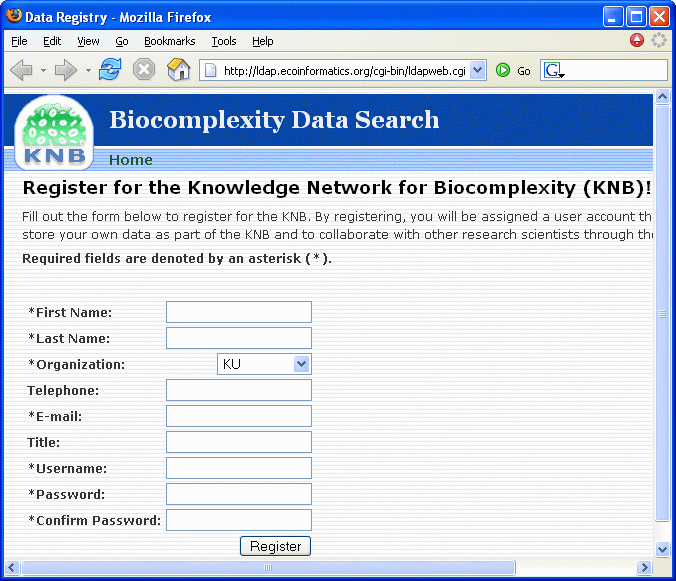
\includegraphics[width=0.7\textwidth]{images/register-knb.png}
  \caption{Registering for the KNB network}
  \label{fig:register-knb}
\end{figure}

\subsubsection{Create a User Profile}

The user profile allows you to use Morpho locally on your personal
computer and, once registered for the KNB (see \ref{sec:register}), to
create, access, edit, and search for metadata and data on the KNB. 

First-time users will automatically be prompted to create a new profile
when they open Morpho. Users upgrading Morpho from a previous version
may also be prompted to create a new profile. To continue using your
old profile(s) (so that your locally-stored data continue to be
visible), simply enter a ``new profile'' with the same user name as the
old one (e.g., if your old profile is named ``jdoe'', then enter
``jdoe'' as the name of the new profile). Click ``Yes'' when prompted,
to confirm that you would like to use the existing profile. Note: You
must be logged in to your computer with the same account under which
your old profile existed.

\paragraph{To create a user profile:}
\begin{enumerate}
  \item On the ``Basic Information'' screen of the New Profile wizard
    (\autoref{fig:new-profile-name}), enter your profile name and your
    first and last names. Your profile name does \emph{not} have to be
    the same as your KNB username. Click ``Next.''

  \begin{figure}
    \centering
      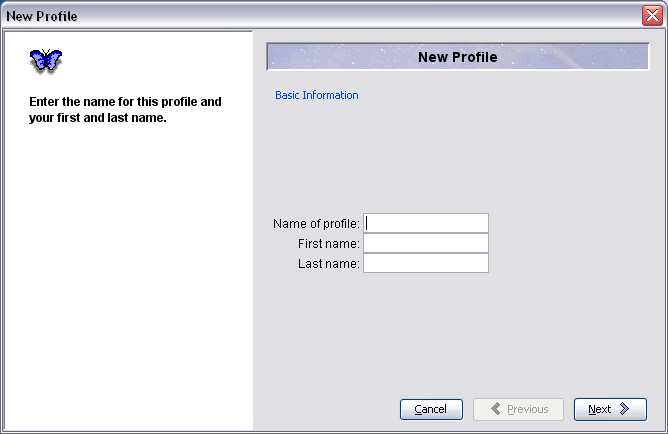
\includegraphics[width=0.7\textwidth]{images/new-profile-name.png}
    \caption{Step 1: Create a profile name.}
    \label{fig:new-profile-name}
  \end{figure}

  \item On the ``Network Account Information'' screen
    (\autoref{fig:new-profile-account}), enter your KNB username and the
    organization you selected when you
    \hyperref[sec:register]{registered for the KNB}. If your
    organization is not listed, click the Refresh button to look up the
    most recent account information. Click ``Next.'' 

  \begin{figure}
    \centering
      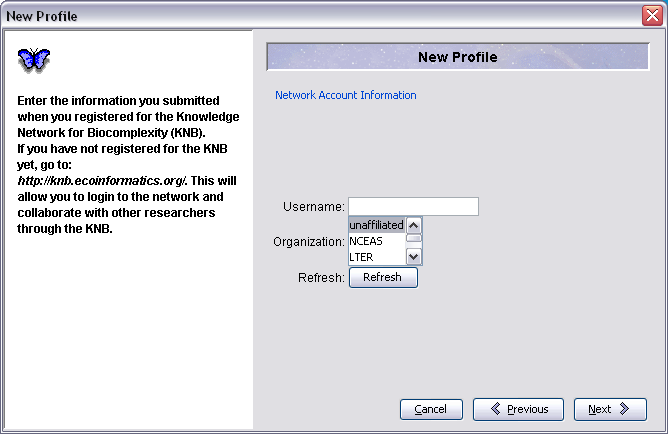
\includegraphics[width=0.7\textwidth]{images/new-profile-account.png}
    \caption{Step 2: Enter your KNB username and organization.}
    \label{fig:new-profile-account}
  \end{figure}

  \item On the ``Data Package Identification'' screen
    (\autoref{fig:new-profile-prefix}), enter a short identifier prefix.
    The identifier prefix will be used to create IDs for metadata
    documents you create in Morpho, and for data tables or other data
    files you import using Morpho. For example, specifying the prefix
    ``jane\_doe'' will result in document IDs like jane\_doe.1.1,
    jane\_doe.2.1, etc. \emph{\textbf{Do not use the reserved prefix
    ``temporary''.}} Other non-alphanumeric characters like periods, 
    commas, and quotation marks are also not allowed in the prefix.

  \begin{figure}
    \centering
      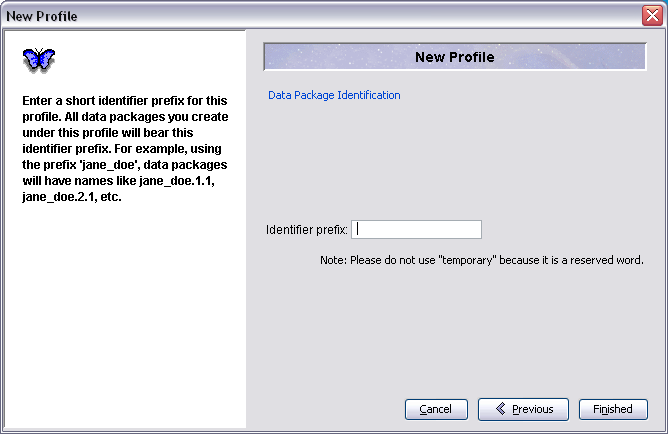
\includegraphics[width=0.7\textwidth]{images/new-profile-prefix.png}
    \caption{Step 3: Specify an identifier prefix.}
    \label{fig:new-profile-prefix}
  \end{figure}

  \item Click ``Finished'' to complete the profile.
\end{enumerate}

\begin{shaded}
  \textbf{NOTE} The Morpho interface currently supports deleting
  profiles that you no longer need through the Remove Profile menu item
  from the File menu (see \autoref{sec:removing-a-profile}).
   \textbf{However, if you delete a profile, you also
  delete all local copies of data packages created or saved using that
  profile}. Unless you first extract the data packages and save them
  elsewhere on your computer (or to a network server, like Metacat), you
  may lose data.
\end{shaded}

\subsection{Logging In}

After you have created a user profile (see
\autoref{sec:before-you-begin}), you will see the Main Morpho screen.
Enter your KNB password in the ``Network Status'' panel and click
``Login'' (\autoref{fig:panel-login}). If you choose not to log in, you
will be able to create, edit, search, access, and manage data that are
stored locally, and may search for public data sets on the KNB network.
However, you will not be allowed to create or edit data sets on the KNB
network.

\begin{figure}
  \centering
    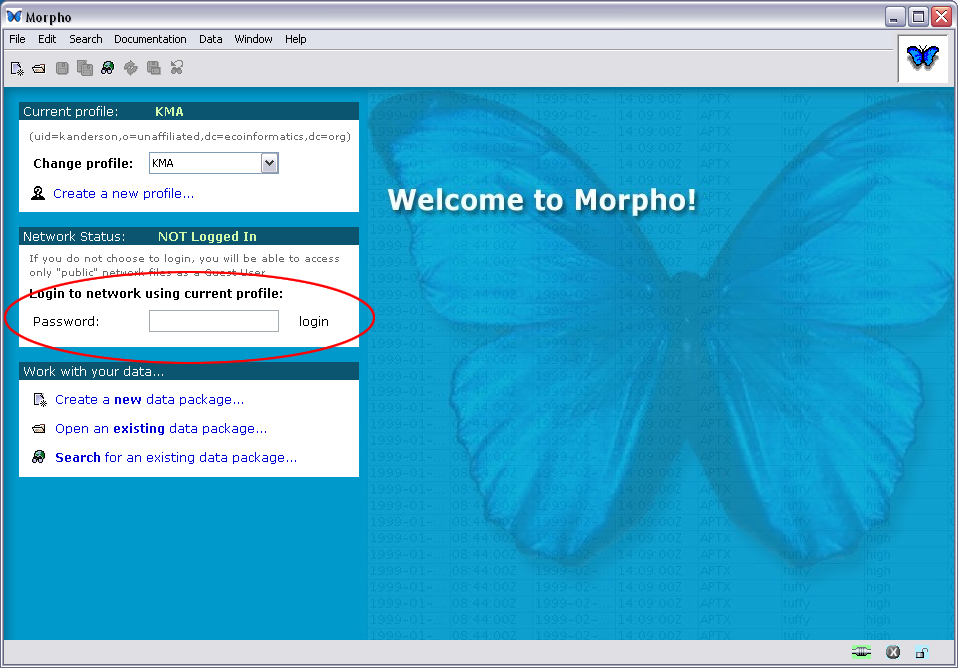
\includegraphics[width=0.7\textwidth]{images/panel-login.jpg}
  \caption{Log in to the KNB network.}
  \label{fig:panel-login}
\end{figure}

\subsection{Removing a profile} \label{sec:removing-a-profile}

Profiles may be removed from Morpho if they are no longer needed.
When you remove a profile, all the metadata and data that has been created 
with that profile is deleted locally. Network copies remain untouched.

\paragraph{To remove a user profile:}
\begin{enumerate}
  \item From the File menu, choose ``Remove profile''
  \item Select the profile that should be removed (\autoref{fig:remove-profile-select}).
  Note: The current active profile cannot be removed (switch to a different profile in order to remove it).
  
  
  \begin{figure}
  \centering
    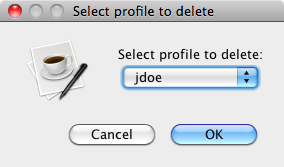
\includegraphics[width=0.7\textwidth]{images/remove-profile-select.png}
  \caption{Select profile to remove}
  \label{fig:remove-profile-select}
\end{figure}
  
  \item Confirm the removal in the dialog box (\autoref{fig:remove-profile-confirm}).
  \begin{figure}
  \centering
    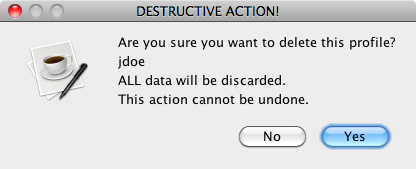
\includegraphics[width=0.7\textwidth]{images/remove-profile-confirm.png}
  \caption{Confirm profile removal.}
  \label{fig:remove-profile-confirm}
\end{figure}

\end{enumerate}

